\documentclass{standalone}
\usepackage{tikz}
\usetikzlibrary{patterns, positioning}


\begin{document}
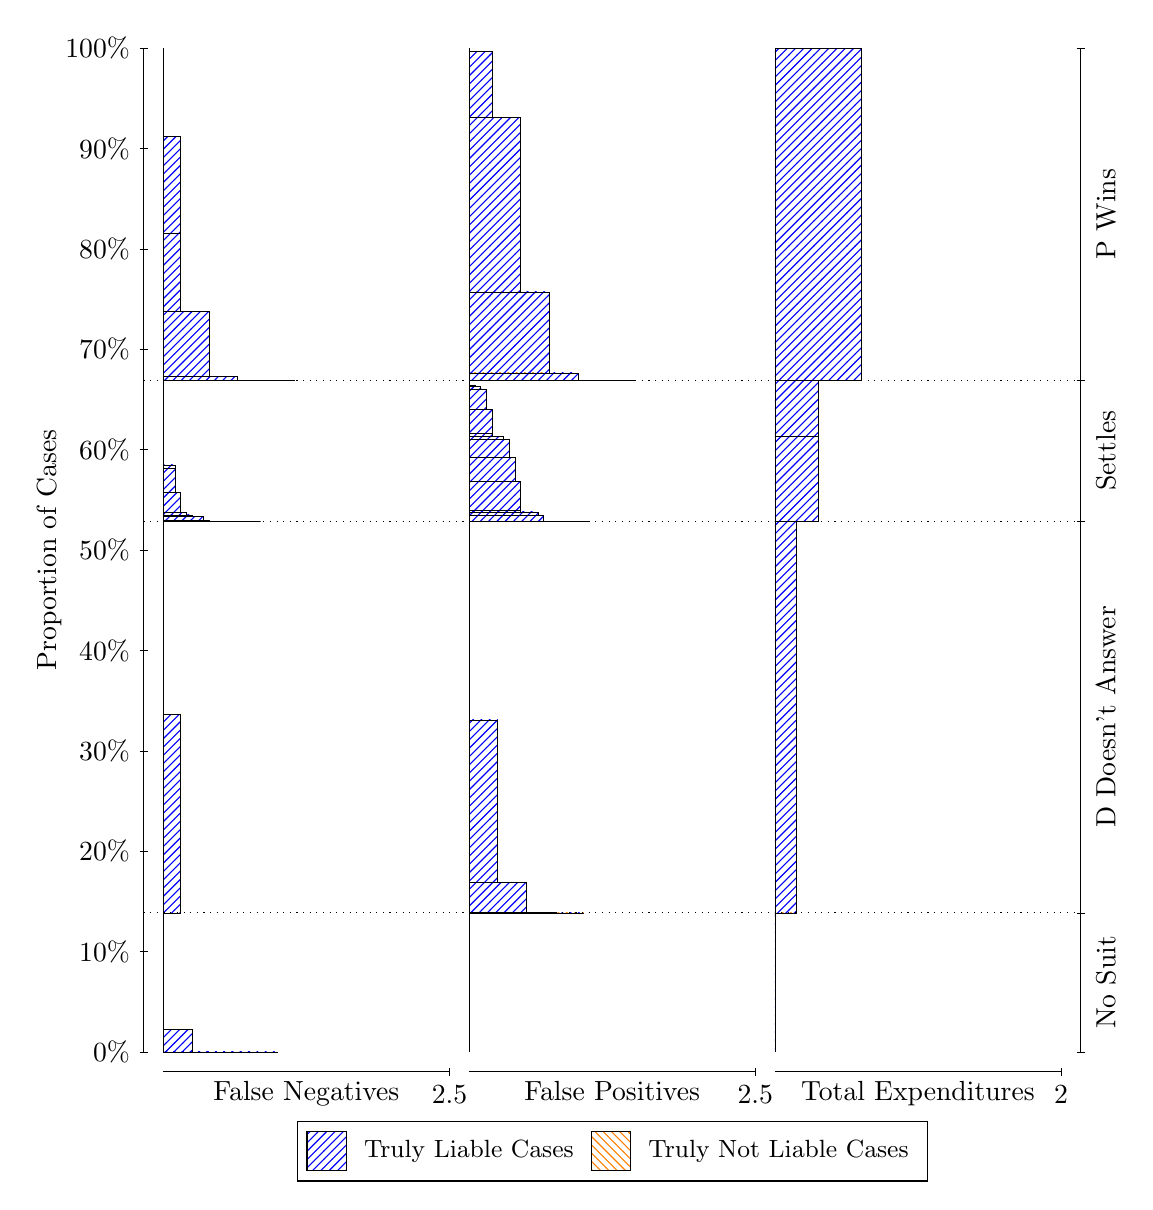
\begin{tikzpicture}
\draw[black, very thin] (1.5,1.75) -- (1.5,14.5);
\node[rotate=90, text=black, anchor=center] at (0.3, 8.125) {Proportion of Cases};
\draw[black, very thin] (1.45,1.75) -- (1.55,1.75);
\node[text=black, anchor=east] at (1.45, 1.75) {0\%};
\draw[black, very thin] (1.45,3.025) -- (1.55,3.025);
\node[text=black, anchor=east] at (1.45, 3.025) {10\%};
\draw[black, very thin] (1.45,4.3) -- (1.55,4.3);
\node[text=black, anchor=east] at (1.45, 4.3) {20\%};
\draw[black, very thin] (1.45,5.575) -- (1.55,5.575);
\node[text=black, anchor=east] at (1.45, 5.575) {30\%};
\draw[black, very thin] (1.45,6.85) -- (1.55,6.85);
\node[text=black, anchor=east] at (1.45, 6.85) {40\%};
\draw[black, very thin] (1.45,8.125) -- (1.55,8.125);
\node[text=black, anchor=east] at (1.45, 8.125) {50\%};
\draw[black, very thin] (1.45,9.4) -- (1.55,9.4);
\node[text=black, anchor=east] at (1.45, 9.4) {60\%};
\draw[black, very thin] (1.45,10.675) -- (1.55,10.675);
\node[text=black, anchor=east] at (1.45, 10.675) {70\%};
\draw[black, very thin] (1.45,11.95) -- (1.55,11.95);
\node[text=black, anchor=east] at (1.45, 11.95) {80\%};
\draw[black, very thin] (1.45,13.225) -- (1.55,13.225);
\node[text=black, anchor=east] at (1.45, 13.225) {90\%};
\draw[black, very thin] (1.45,14.5) -- (1.55,14.5);
\node[text=black, anchor=east] at (1.45, 14.5) {100\%};

\draw[black, very thin] (13.4,1.75) -- (13.4,14.5);
\draw[black, very thin] (13.35,1.75) -- (13.45,1.75);
\node[anchor=west] at (13.35, 1.75) {};
\draw[black, very thin] (13.35,3.5173) -- (13.45,3.5173);
\node[anchor=west] at (13.35, 3.5173) {};
\draw[black, very thin] (13.35,8.4916) -- (13.45,8.4916);
\node[anchor=west] at (13.35, 8.4916) {};
\draw[black, very thin] (13.35,10.282) -- (13.45,10.282);
\node[anchor=west] at (13.35, 10.282) {};
\draw[black, very thin] (13.35,14.5) -- (13.45,14.5);
\node[anchor=west] at (13.35, 14.5) {};

\draw[black, very thin, pattern color=blue, pattern=north east lines] (1.75,1.75) rectangle (3.2033,1.75);
\draw[black, very thin, pattern color=blue, pattern=north east lines] (1.75,1.75) rectangle (2.84,1.75);
\draw[black, very thin, pattern color=blue, pattern=north east lines] (1.75,1.75) rectangle (2.4767,1.7525);
\draw[black, very thin, pattern color=blue, pattern=north east lines] (1.75,1.7525) rectangle (2.1133,2.0394);
\draw[black, very thin, pattern color=orange, pattern=north west lines] (1.75,2.0394) rectangle (1.75,2.0394);
\draw[black, very thin, pattern color=blue, pattern=north east lines] (1.75,2.0394) rectangle (1.75,3.5173);
\draw[black, very thin, pattern color=blue, pattern=north east lines] (1.75,3.5173) rectangle (1.968,6.0407);
\draw[black, very thin, pattern color=orange, pattern=north west lines] (1.75,6.0407) rectangle (1.75,6.0407);
\draw[black, very thin, pattern color=blue, pattern=north east lines] (1.75,6.0407) rectangle (1.75,8.4916);
\draw[black, very thin, pattern color=blue, pattern=north east lines] (1.75,8.4916) rectangle (2.9853,8.4916);
\draw[black, very thin, pattern color=blue, pattern=north east lines] (1.75,8.4916) rectangle (2.6947,8.4916);
\draw[black, very thin, pattern color=blue, pattern=north east lines] (1.75,8.4916) rectangle (2.622,8.4917);
\draw[black, very thin, pattern color=blue, pattern=north east lines] (1.75,8.4917) rectangle (2.404,8.4918);
\draw[black, very thin, pattern color=blue, pattern=north east lines] (1.75,8.4918) rectangle (2.3313,8.501);
\draw[black, very thin, pattern color=blue, pattern=north east lines] (1.75,8.501) rectangle (2.2587,8.5518);
\draw[black, very thin, pattern color=blue, pattern=north east lines] (1.75,8.5518) rectangle (2.1133,8.5721);
\draw[black, very thin, pattern color=blue, pattern=north east lines] (1.75,8.5721) rectangle (2.0407,8.6015);
\draw[black, very thin, pattern color=blue, pattern=north east lines] (1.75,8.6015) rectangle (1.968,8.8589);
\draw[black, very thin, pattern color=blue, pattern=north east lines] (1.75,8.8589) rectangle (1.8953,9.1649);
\draw[black, very thin, pattern color=blue, pattern=north east lines] (1.75,9.1649) rectangle (1.8953,9.207);
\draw[black, very thin, pattern color=orange, pattern=north west lines] (1.75,9.207) rectangle (1.75,9.207);
\draw[black, very thin, pattern color=blue, pattern=north east lines] (1.75,9.207) rectangle (1.75,10.282);
\draw[black, very thin, pattern color=blue, pattern=north east lines] (1.75,10.282) rectangle (3.4213,10.282);
\draw[black, very thin, pattern color=blue, pattern=north east lines] (1.75,10.282) rectangle (3.058,10.282);
\draw[black, very thin, pattern color=blue, pattern=north east lines] (1.75,10.282) rectangle (2.6947,10.327);
\draw[black, very thin, pattern color=blue, pattern=north east lines] (1.75,10.327) rectangle (2.3313,11.16);
\draw[black, very thin, pattern color=blue, pattern=north east lines] (1.75,11.16) rectangle (1.968,12.145);
\draw[black, very thin, pattern color=blue, pattern=north east lines] (1.75,12.145) rectangle (1.968,13.379);
\draw[black, very thin, pattern color=orange, pattern=north west lines] (1.75,13.379) rectangle (1.75,13.379);
\draw[black, very thin, pattern color=blue, pattern=north east lines] (1.75,13.379) rectangle (1.75,14.5);
\draw[black, very thin, pattern color=orange, pattern=north west lines] (5.6333,1.75) rectangle (5.6333,1.75);
\draw[black, very thin, pattern color=blue, pattern=north east lines] (5.6333,1.75) rectangle (5.6333,3.5173);
\draw[black, very thin, pattern color=orange, pattern=north west lines] (5.6333,3.5173) rectangle (7.0867,3.5173);
\draw[black, very thin, pattern color=blue, pattern=north east lines] (5.6333,3.5173) rectangle (7.0867,3.5173);
\draw[black, very thin, pattern color=blue, pattern=north east lines] (5.6333,3.5173) rectangle (6.7233,3.5203);
\draw[black, very thin, pattern color=blue, pattern=north east lines] (5.6333,3.5203) rectangle (6.36,3.9056);
\draw[black, very thin, pattern color=blue, pattern=north east lines] (5.6333,3.9056) rectangle (5.9967,5.9683);
\draw[black, very thin, pattern color=blue, pattern=north east lines] (5.6333,5.9683) rectangle (5.6333,8.4916);
\draw[black, very thin, pattern color=orange, pattern=north west lines] (5.6333,8.4916) rectangle (7.1593,8.4916);
\draw[black, very thin, pattern color=blue, pattern=north east lines] (5.6333,8.4916) rectangle (7.1593,8.4916);
\draw[black, very thin, pattern color=orange, pattern=north west lines] (5.6333,8.4916) rectangle (7.014,8.4916);
\draw[black, very thin, pattern color=blue, pattern=north east lines] (5.6333,8.4916) rectangle (7.014,8.4916);
\draw[black, very thin, pattern color=orange, pattern=north west lines] (5.6333,8.4916) rectangle (6.8687,8.4916);
\draw[black, very thin, pattern color=blue, pattern=north east lines] (5.6333,8.4916) rectangle (6.8687,8.4918);
\draw[black, very thin, pattern color=blue, pattern=north east lines] (5.6333,8.4918) rectangle (6.796,8.4918);
\draw[black, very thin, pattern color=blue, pattern=north east lines] (5.6333,8.4918) rectangle (6.6507,8.4919);
\draw[black, very thin, pattern color=orange, pattern=north west lines] (5.6333,8.4919) rectangle (6.578,8.4919);
\draw[black, very thin, pattern color=blue, pattern=north east lines] (5.6333,8.4919) rectangle (6.578,8.5606);
\draw[black, very thin, pattern color=blue, pattern=north east lines] (5.6333,8.5606) rectangle (6.5053,8.6089);
\draw[black, very thin, pattern color=blue, pattern=north east lines] (5.6333,8.6089) rectangle (6.4327,8.6104);
\draw[black, very thin, pattern color=blue, pattern=north east lines] (5.6333,8.6104) rectangle (6.2873,8.6278);
\draw[black, very thin, pattern color=orange, pattern=north west lines] (5.6333,8.6278) rectangle (6.2873,8.6278);
\draw[black, very thin, pattern color=blue, pattern=north east lines] (5.6333,8.6278) rectangle (6.2873,8.9915);
\draw[black, very thin, pattern color=blue, pattern=north east lines] (5.6333,8.9915) rectangle (6.2147,9.2975);
\draw[black, very thin, pattern color=blue, pattern=north east lines] (5.6333,9.2975) rectangle (6.142,9.5266);
\draw[black, very thin, pattern color=blue, pattern=north east lines] (5.6333,9.5266) rectangle (6.0693,9.5667);
\draw[black, very thin, pattern color=blue, pattern=north east lines] (5.6333,9.5667) rectangle (5.924,9.6088);
\draw[black, very thin, pattern color=blue, pattern=north east lines] (5.6333,9.6088) rectangle (5.924,9.9148);
\draw[black, very thin, pattern color=blue, pattern=north east lines] (5.6333,9.9148) rectangle (5.8513,10.172);
\draw[black, very thin, pattern color=blue, pattern=north east lines] (5.6333,10.172) rectangle (5.7787,10.202);
\draw[black, very thin, pattern color=blue, pattern=north east lines] (5.6333,10.202) rectangle (5.706,10.222);
\draw[black, very thin, pattern color=blue, pattern=north east lines] (5.6333,10.222) rectangle (5.6333,10.282);
\draw[black, very thin, pattern color=orange, pattern=north west lines] (5.6333,10.282) rectangle (7.7407,10.282);
\draw[black, very thin, pattern color=blue, pattern=north east lines] (5.6333,10.282) rectangle (7.7407,10.282);
\draw[black, very thin, pattern color=orange, pattern=north west lines] (5.6333,10.282) rectangle (7.3773,10.282);
\draw[black, very thin, pattern color=blue, pattern=north east lines] (5.6333,10.282) rectangle (7.3773,10.283);
\draw[black, very thin, pattern color=orange, pattern=north west lines] (5.6333,10.283) rectangle (7.014,10.283);
\draw[black, very thin, pattern color=blue, pattern=north east lines] (5.6333,10.283) rectangle (7.014,10.375);
\draw[black, very thin, pattern color=orange, pattern=north west lines] (5.6333,10.375) rectangle (6.6507,10.375);
\draw[black, very thin, pattern color=blue, pattern=north east lines] (5.6333,10.375) rectangle (6.6507,11.403);
\draw[black, very thin, pattern color=orange, pattern=north west lines] (5.6333,11.403) rectangle (6.2873,11.403);
\draw[black, very thin, pattern color=blue, pattern=north east lines] (5.6333,11.403) rectangle (6.2873,13.622);
\draw[black, very thin, pattern color=blue, pattern=north east lines] (5.6333,13.622) rectangle (5.924,14.455);
\draw[black, very thin, pattern color=blue, pattern=north east lines] (5.6333,14.455) rectangle (5.6333,14.5);
\draw[black, very thin, pattern color=orange, pattern=north west lines] (9.5167,1.75) rectangle (9.5167,1.75);
\draw[black, very thin, pattern color=blue, pattern=north east lines] (9.5167,1.75) rectangle (9.5167,3.5173);
\draw[black, very thin, pattern color=orange, pattern=north west lines] (9.5167,3.5173) rectangle (9.7892,3.5173);
\draw[black, very thin, pattern color=blue, pattern=north east lines] (9.5167,3.5173) rectangle (9.7892,8.4916);
\draw[black, very thin, pattern color=orange, pattern=north west lines] (9.5167,8.4916) rectangle (10.062,8.4916);
\draw[black, very thin, pattern color=blue, pattern=north east lines] (9.5167,8.4916) rectangle (10.062,9.5636);
\draw[black, very thin, pattern color=orange, pattern=north west lines] (9.5167,9.5636) rectangle (10.062,9.5636);
\draw[black, very thin, pattern color=blue, pattern=north east lines] (9.5167,9.5636) rectangle (10.062,10.282);
\draw[black, very thin, pattern color=orange, pattern=north west lines] (9.5167,10.282) rectangle (10.607,10.282);
\draw[black, very thin, pattern color=blue, pattern=north east lines] (9.5167,10.282) rectangle (10.607,14.5);
\draw[black, dotted] (1.5,3.5173) -- (13.4,3.5173);
\draw[black, dotted] (1.5,8.4916) -- (13.4,8.4916);
\draw[black, dotted] (1.5,10.282) -- (13.4,10.282);
\draw[black, very thin] (1.75,1.5) -- (5.3833,1.5);
\node[text=black, anchor=north] at (3.5667, 1.5) {False Negatives};
\draw[black, very thin] (5.3833,1.45) -- (5.3833,1.55);
\node[text=black, anchor=north] at (5.3833, 1.45) {2.5};

\draw[black, very thin] (5.6333,1.5) -- (9.2667,1.5);
\node[text=black, anchor=north] at (7.45, 1.5) {False Positives};
\draw[black, very thin] (9.2667,1.45) -- (9.2667,1.55);
\node[text=black, anchor=north] at (9.2667, 1.45) {2.5};

\draw[black, very thin] (9.5167,1.5) -- (13.15,1.5);
\node[text=black, anchor=north] at (11.333, 1.5) {Total Expenditures};
\draw[black, very thin] (13.15,1.45) -- (13.15,1.55);
\node[text=black, anchor=north] at (13.15, 1.45) {2};

\node[text=black, centered, rotate=90] at (13.72, 2.6337) {No Suit};
\node[text=black, centered, rotate=90] at (13.72, 6.0045) {D Doesn't Answer};
\node[text=black, centered, rotate=90] at (13.72, 9.3868) {Settles};
\node[text=black, centered, rotate=90] at (13.72, 12.391) {P Wins};

\draw (7.449999999999999,1.5) node[draw=none] (baseCoordinate) {};
\begin{scope}[align=center]
        \matrix[scale=0.5, draw=black, below=0.5cm of baseCoordinate, nodes={draw}, column sep=0.1cm]{
            \node[rectangle, draw, minimum width=0.5cm, minimum height=0.5cm, pattern color=blue, pattern=north east lines] {}; &
            \node[draw=none, font=\small, text=black] (B) {Truly Liable Cases}; &
            \node[rectangle, draw, minimum width=0.5cm, minimum height=0.5cm, pattern color=orange, pattern=north west lines] {}; &
            \node[draw=none, font=\small, text=black] (B) {Truly Not Liable Cases}; \\
            };
\end{scope}

\end{tikzpicture}
\end{document}